%% ============================================================
%% tex/decay_schemes.tex
%% Decay-scheme row aligned to the three panels of images/spectra.pdf.
%% Input directly below 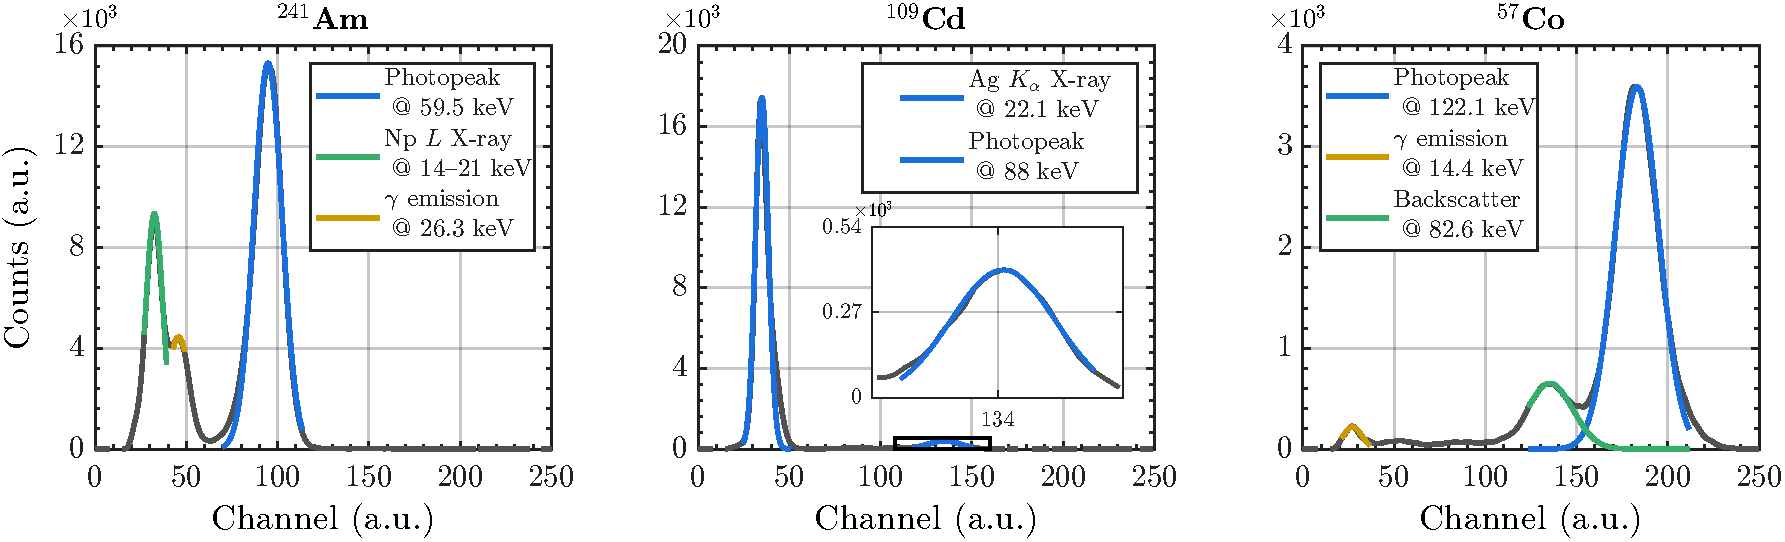
\includegraphics[width=\linewidth]{images/spectra.pdf}.
%% Requires only \usepackage{tikz}.
%% ============================================================
\usetikzlibrary{arrows.meta}
\begingroup

%% ---- panel geometry, as fractions of \linewidth --------------------
%% Measured from the current spectra.pdf (default MATLAB subplot
%% positions, tight crop). If the figure is regenerated with the pinned
%% panel grid and exportgraphics(...,'Padding','figure'), comment this
%% block and uncomment the one below it.
\def\dsBoxW{0.2818}
\def\dsCA{0.1801}
\def\dsCB{0.5191}
\def\dsCC{0.8592}
% \def\dsBoxW{0.2880}
% \def\dsCA{0.204667}
% \def\dsCB{0.530000}
% \def\dsCC{0.855333}

\definecolor{dsblue}{RGB}{26,111,223}      % alpha
\definecolor{dsgreen}{RGB}{55,173,107}     % electron capture
\definecolor{dsyellow}{RGB}{204,153,0}     % gamma
\definecolor{dsgrey}{RGB}{81,81,81}        % levels
\definecolor{dsdark}{RGB}{40,40,40}        % text

%% parent bar: #1 nuclide, #2 half-life
\def\dsParent#1#2{%
  \draw[dslvl] (34,120) -- (60,120);
  \node[dslbl,  anchor=south] at (47,121.5) {#1};
  \node[dsslab, anchor=east]  at (60,115)   {#2};}

%% decay branch: #1 colour, #2 target level, #3 label above, #4 label below
\def\dsBranch#1#2#3#4{%
  \draw[dsarr, #1] (34,120) -- (14,#2);
  \node[dsslab, anchor=east] at (26,116) {#3};
  \node[dsslab, anchor=west] at (26,99)  {#4};}

%% level: #1 height, #2 energy label
\def\dsLev#1#2{%
  \draw[dslvl] (-29,#1) -- (14,#1);
  \node[dsslab, anchor=east] at (-31,#1) {#2};}

%% gamma transition, unlabelled: #1 x, #2 from, #3 to
\def\dsGam#1#2#3{\draw[dsarr, dsyellow] (#1,#2) -- (#1,#3);}

%% gamma transition, labelled horizontally: #1 x, #2 from, #3 to, #4 label
\def\dsGamL#1#2#3#4{%
  \draw[dsarr, dsyellow] (#1,#2) -- (#1,#3);
  \node[dsslab, anchor=west] at ({#1+4},{(#2+#3)/2}) {#4};}

\def\dsProd#1{\node[dslbl, anchor=north] at (-7,26) {#1};}
\def\dsLetter#1{\node[dsltr, anchor=south] at (0,0) {#1};}

\pgfmathsetmacro{\dsLW}{\linewidth/1pt}
\pgfmathsetmacro{\dsPS}{\dsBoxW*\dsLW/120}
\pgfmathsetmacro{\dsHT}{134*\dsPS}
\pgfmathsetmacro{\dsA}{\dsCA*\dsLW}
\pgfmathsetmacro{\dsB}{\dsCB*\dsLW}
\pgfmathsetmacro{\dsC}{\dsCC*\dsLW}

\begin{tikzpicture}[
    x=1pt, y=1pt,
    dslvl/.style  = {dsgrey, line width=0.7pt},
    dsarr/.style  = {-{Stealth[length=3.6pt,width=2.7pt]}, line width=0.8pt},
    dslbl/.style  = {font=\scriptsize,     text=dsdark, inner sep=0.8pt},
    dsslab/.style = {font=\tiny,           text=dsdark, inner sep=0.6pt},
    dsltr/.style  = {font=\small\bfseries, text=dsdark, inner sep=0pt}]

  \useasboundingbox (0,0) rectangle (\dsLW,\dsHT);

  % Alignment check: uncomment to rule through each panel centre.
  % \foreach \f in {\dsCA,\dsCB,\dsCC}
  %   {\draw[red, line width=0.2pt] ({\f*\dsLW},0) -- ({\f*\dsLW},\dsHT);}

  %% ---- (a) Am-241 --------------------------------------------------
  \begin{scope}[overlay, shift={(\dsA,0)}, scale=\dsPS]
    \dsParent{$^{241}$Am}{432.6\,y}
    \dsBranch{dsblue}{84}{$\alpha$}{85.2\%}
    \dsLev{84}{59.5\,keV}
    \dsLev{58}{33.2\,keV}
    \dsLev{34}{0\,keV}
    \dsGam{-22}{84}{34}
    \dsGamL{-8}{84}{58}{26.3\,keV}
    \dsGam{8}{58}{34}
    \dsProd{$^{237}$Np}
    \dsLetter{(a)}
  \end{scope}

  %% ---- (b) Cd-109 --------------------------------------------------
  \begin{scope}[overlay, shift={(\dsB,0)}, scale=\dsPS]
    \dsParent{$^{109}$Cd}{461.4\,d}
    \dsBranch{dsgreen}{84}{EC}{100\%}
    \dsLev{84}{88\,keV}
    \dsLev{34}{0\,keV}
    \dsGam{-7}{84}{34}
    \dsProd{$^{109}$Ag}
    \dsLetter{(b)}
  \end{scope}

  %% ---- (c) Co-57 ---------------------------------------------------
  \begin{scope}[overlay, shift={(\dsC,0)}, scale=\dsPS]
    \dsParent{$^{57}$Co}{271.7\,d}
    \dsBranch{dsgreen}{92}{EC}{99.8\%}
    \dsLev{92}{136.5\,keV}
    \dsLev{50}{14.4\,keV}
    \dsLev{34}{0\,keV}
    \dsGam{-24}{92}{34}
    \dsGamL{-10}{92}{50}{122.1\,keV}
    \dsGam{4}{50}{34}
    \dsProd{$^{57}$Fe}
    \dsLetter{(c)}
  \end{scope}
\end{tikzpicture}
\endgroup%